% ======================================================================
% col: 20
\chapter{Introduzione}

\section{F1TENTH}
F1TENTH è una community internazionale di ricercatori, ingegneri e appassionati di sistemi autonomi
che organizza competizioni di corsa di macchinine con la peculiare caratteristica
di essere \textit{un decimo} di quelle di F1, da cui il nome.
\begin{wrapfigure}{r}{0.3\textwidth}
	\centering
	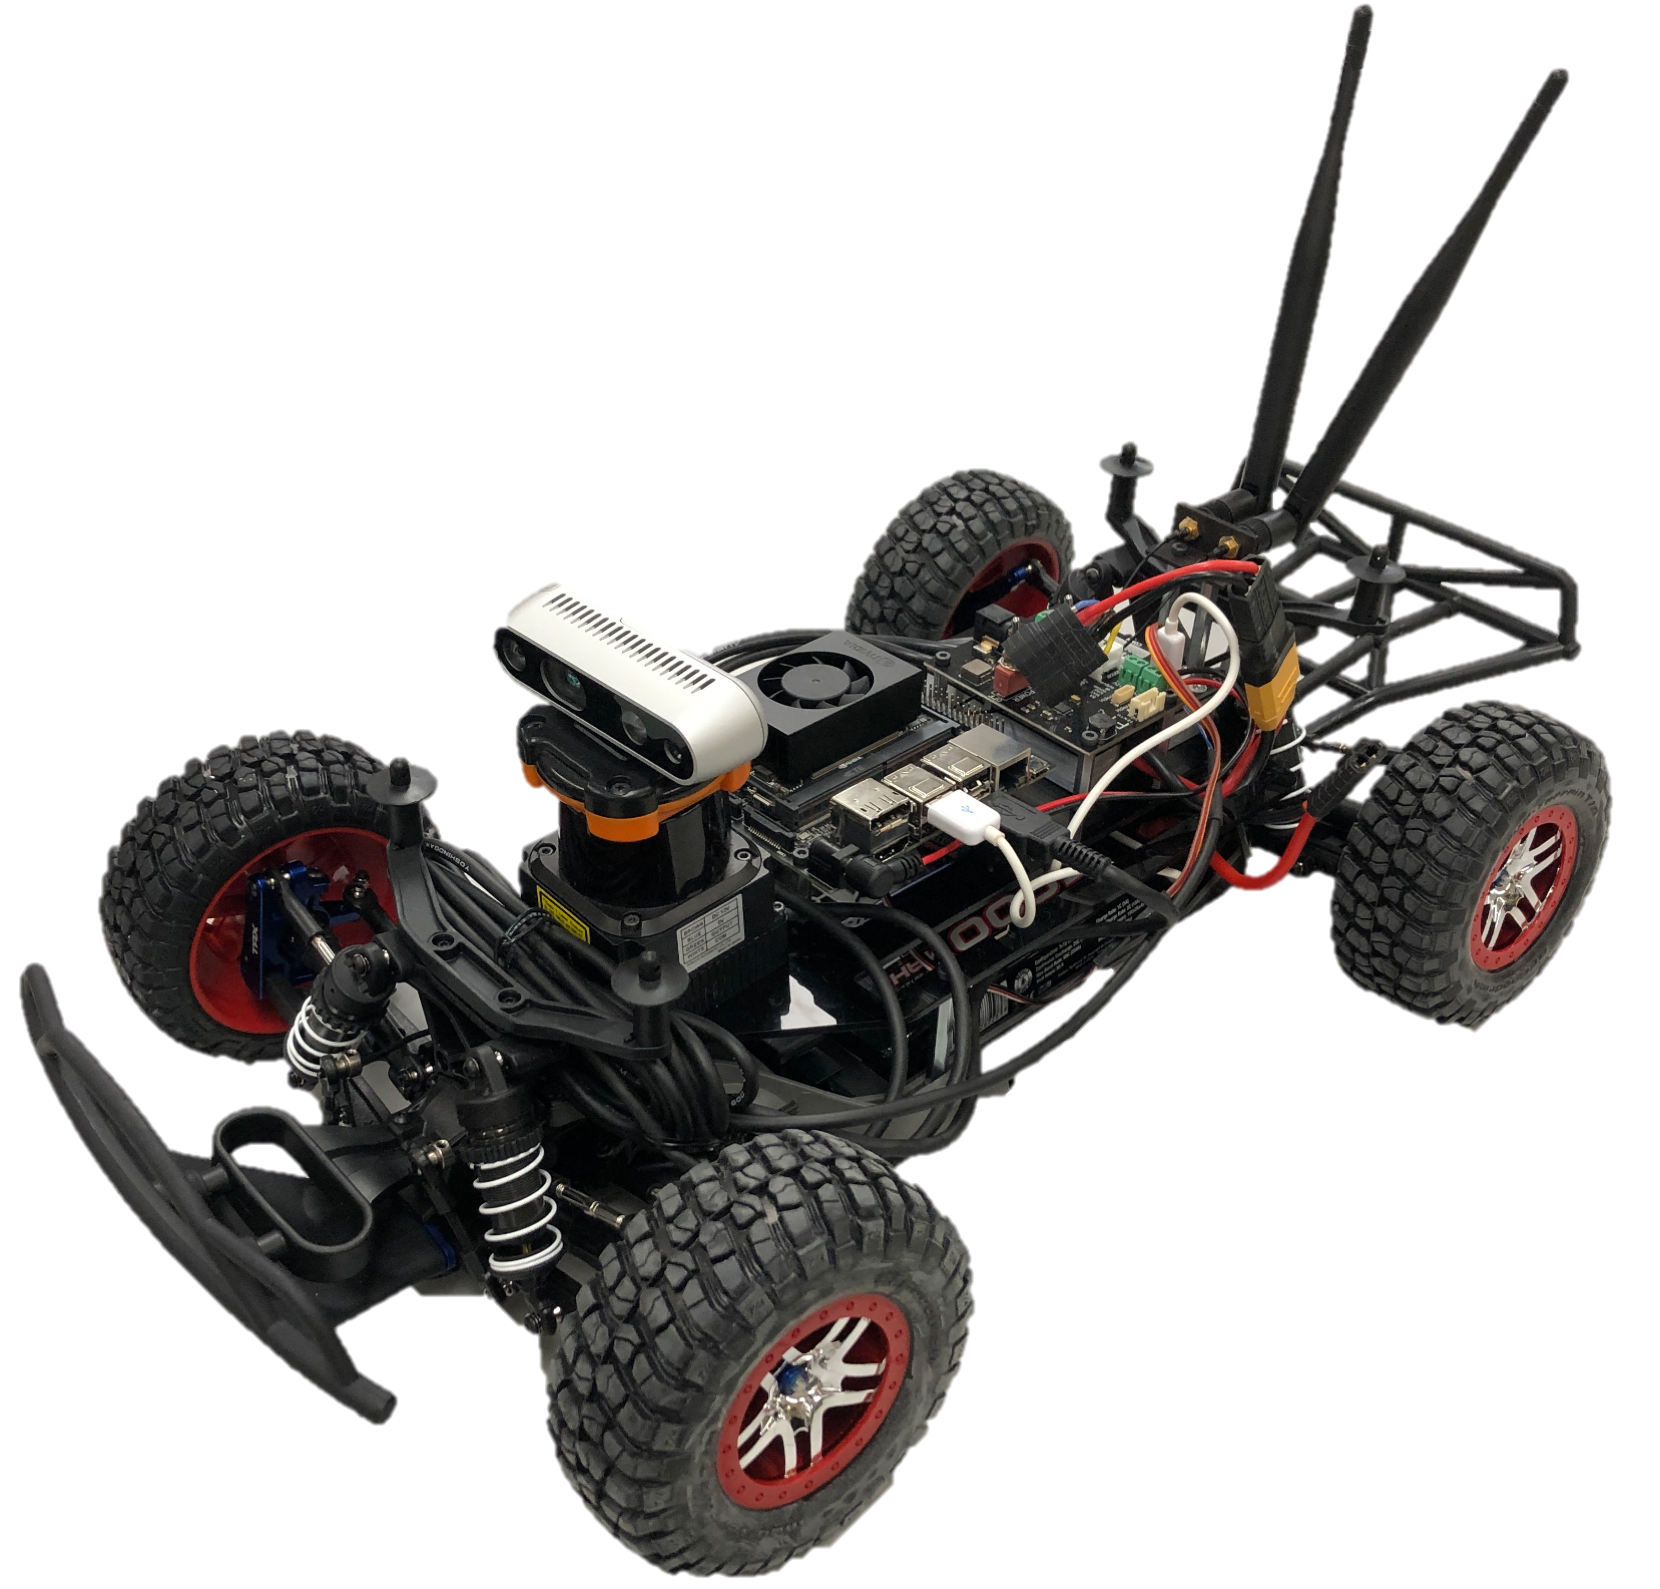
\includegraphics[width=0.2\textwidth]{f1tenth-car.png}
	{\footnotesize Macchinina di F1TENTH}
\end{wrapfigure}
Oltre a questo, promuove la ricerca nell'ambito della guida autonoma
e altri campi tra cui reinforcement learning, sistemi di comunicazione e robotica;
offre, inoltre, corsi gratuiti online e una infrastuttura per imparare a costruire l'auto da corsa
e sviluppare il software necessario per farla gareggiare. % TODO: \cite{f1tenth}

La community è stata fondata all'Università della Pennsylvania nel 2016 ma ha iniziato rapidamente
collaborazioni con altre istituzioni e università in tutto il mondo~--~in Italia, alla data di stesura, solo
con l'Università degli Studi di Modena e Reggio Emilia.

\paragraph{I corsi}
Il percorso di apprendimento, che ha materiale per un semestre circa
% TODO: \footnote{https://f1tenth.org/learn.html},
raggruppa le lezioni in moduli e li integra con altrettanti laboratori guidati
su cui poter applicare le nozioni e algoritmi imparati.

% TODO: da rivedere per non spaccare la lista in più pagine
% \begin{minipage}{\textwidth}
\noindent I moduli si raggruppano per tipologia di argomento trattato:
\begin{itemize}
	%TODO: breve descrizione dei contenuti
	\item \textit{Modulo A} -- Introduzione a Robot Operating System (ROS) e \\
	      all'ambiente simulatore di F1TENTH gym;
	\item \textit{Modulo B} -- Metodi reattivi e dinamiche del veicolo
	\item \textit{Modulo C} -- Mapping \& Localization: SLAM e Particle Filter;
	\item \textit{Modulo D} -- Planning \& Control: Pure Pursuit e RRT;
	\item \textit{Modulo E} -- Vision
	\item \textit{Modulo F} -- Argomenti speciali: \textit{Raceline Optimization}, MPC
	\item \textit{Modulo G} -- Gareggiare
\end{itemize}
% \end{minipage} \\

\noindent Ai fini dell'obiettivo di questa tesi, si è preferito non approfondire il Modulo E,
oltre al fatto che si rendeva
necessario l'uso fisico di hardware di cui non si aveva accesso,
ovvero l'auto e soprattutto sensori di visione come telecamere e LiDAr.

\paragraph{F1TENTH gym}
% TODO: da rivedere
% https://docs.google.com/presentation/d/1zfzzjVTbXNIZ75BFtGEwQBJRHlY95VKkFQjJhYfznpI/edit#slide=id.g1cca33b1c19_0_3213
La community sviluppa e mantiene un simulatore open-source specifico per F1TENTH
% \footnote{https://github.com/f1tenth/f1tenth_gym_ros},
in modo da poter sviluppare e testare comodamente
senza l'uso di hardware specifico definito per la costruzione della macchinina.\\
Il simulatore definisce la dinamica del veicolo in modo tale da avere una simulazione
più reale possibile % Sim2Real problem
% e grazie a ROS e rviz (che sta per ROS Visualizer)

\subsection{Laboratori}
% TODO: parlare dei laboratori svolti

% ================== Autonomous Driving Pipeline =======================
\section{Autonomous Driving Pipeline}
Un progetto ben strutturato è più efficiente da mantenere e ha maggiori probabilità
di funzionare correttamente: ciò si applica anche in questo caso.\\
Un progetto complesso come quello dei veicoli autonomi deve essere suddiviso in sotto-problemi
più specifici e in modo tale che composti insieme risultino nella soluzione del problema.
\par

\noindent Il \emph{software} per i veicoli autonomi segue un ciclo di operazioni
in cui il prodotto di una fase è input della successiva; si indentificano in ordine tre fasi:
\begin{enumerate}
	\item \textbf{Perception} Attraverso sensori ottici e radar si \emph{percepisce} il mondo attorno a se,
	      ci si localizza nella mappa e si indentificano eventuali ostacoli o gareggianti
	\item \textbf{Planning} Stando ai dati generati nella fase precedente,
	      si determinano quali saranno le \emph{mosse future} seguendo delle policy prescritte
	\item \textbf{Control} Si generano dei comandi di angolo di sterzata e velocità per attuare le scelte
	      determinate nella fase precedente
\end{enumerate}

L'input per la prima fase (\textit{Perception}) e l'ouput dell'ultima (\textit{Control})
è direttamente l'hardware: dunque nella prima sono i sensori ottici e radar, come citato precedentemente,
mentre nella seconda sono gli attuatori per i controllo della velocità e angolo delle ruote.\par
Il risultato che si vuole ottenere, quindi, è quello di una sequenza di comandi di sterzata e accelerazione
in un contesto, quello delle corse, che richiede una certa velocità di esecuzione per poter essere
il più reattivi possibile, dunque si tende ad eseguire il ciclo tra le 20 e 50 volte al secondo.\\
Una rappresentazione grafica della pipeline intera si trova alla figura \ref{fig:av-pipeline}\\
\begin{figure}[t]
	\centering
	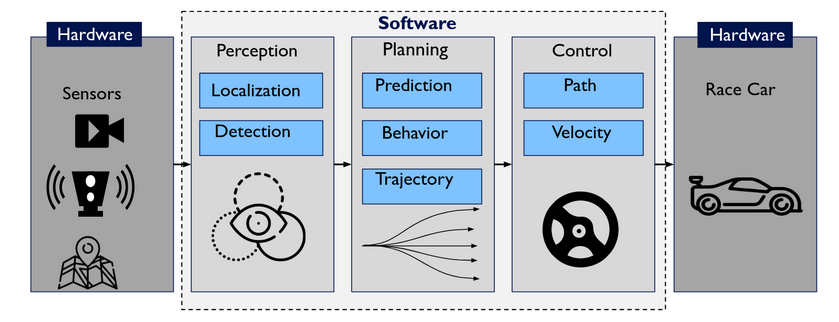
\includegraphics[width=\textwidth]{AV-pipeline.png}
	\caption{Pipeline per i veicolo autonomi}
	\label{fig:av-pipeline}
\end{figure}

Analizziamo più nel dettaglio le fasi sopra citate. % TODO
\paragraph{Perception}

\paragraph{Planning}

\paragraph{Control}

% ================== ROS 2 ================================
\section{ROS2}
% cit: https://docs.ros.org/en/humble/Citations.html
% TODO: da continuare/rivedere
ROS è un acronimo che sta per \textbf{R}obot \textbf{O}perating \textbf{S}ystem e,
sebbene il nome possa trarre in inganno, non è un sistema operativo nel senso tradizionale,
bensì è più simile a un SKD (Software Development Kit).
% https://www.ros.org/blog/ecosystem/
Viene usato da tutta l'industria della robotica: dalla ricerca all'insegnamento, da progetti
di un gruppo di persone a progetti più importanti di grosse aziende.\\
ROS fornisce i \textit{building blocks} da usare per facilitare e velocizzare la realizzazione
del tuo progetto \dots
% TODO: parlare della community e pacchetti 
% TODO: parlare di ros2

ROS si presenta come un mediatore -- un \textbf{middleware} -- tra l'applicazione robot e l'hardware:
alla base fornisce un metodo di comunicazione tra le componenti dell'applicativo chiamati
\textbf{\textit{Nodi}} secondo il pattern \textit{publisher/subscriber} di tipo anonimo.
L'insieme dei nodi e dei loro collegamenti formano il \textit{ROS~Graph}, il grafo dei nodi.
\\

\noindent Di seguito si analizzano le componenti principali di cui ROS è composto.

\paragraph{Nodi}
I nodi, \textit{Nodes} in inglese, sono l'unità computazionale che partecipa al grafo dei nodi;
idealmente, dovrebbero compiere un compito logicamente separato dal resto dei nodi.\\
Essi possono \textit{pubblicare} e \textit{sottoscriversi} a dei \textbf{\textit{Topic}} per inviare e
ricevere dati da altri componenti del grafo.

\paragraph{Topic}
